\documentclass[12pt]{report} % Use report class for chapters
\usepackage[a4paper, margin=1in]{geometry} % Adjust margins
\usepackage{amsmath, amssymb} % For math formatting
\usepackage{titlesec} % For customising section titles
\usepackage{fancyhdr} % For headers and footers
\usepackage{hyperref} % For a clickable table of contents and references
\usepackage{tocloft} % For customising the table of contents
\usepackage{setspace} % For line spacing
\usepackage{graphicx} % For figures and plots
\usepackage{caption} % For custom figure captions
\usepackage{subcaption}
\usepackage{float}
\usepackage[numbers, super]{natbib} % For citation styles
\usepackage{listings}
\lstset{
    basicstyle=\ttfamily,
    language=R
}

% Formatting title sections
\titleformat{\chapter}[hang]{\bfseries\LARGE}{Chapter \thechapter}{1em}{}
\titleformat{\section}[hang]{\large\bfseries}{\thesection}{1em}{}
\titleformat{\subsection}[hang]{\normalsize\bfseries}{\thesubsection}{1em}{}

% Customise TOC spacing
\renewcommand{\cftchapdotsep}{1.5} % Adjust dots in TOC

% Line spacing
\onehalfspacing % Set 1.5 line spacing

% Header and footer
\pagestyle{fancy}
\fancyhf{}
\fancyhead[L]{\slshape \leftmark} % Chapter title on left
\fancyfoot[C]{\thepage} % Page number at center

% Begin document
\begin{document}

% Title page
\begin{titlepage}
    \centering
    {\Huge \textbf{A Bayes Linear Approach to the Branin-Hoo Function}}\\
    \vspace{1cm}
    {\Large \textit{Uncertainty Quantification and Emulator Development}}\\
    \vspace{2cm}
    {\Large \textbf{Raul Unnithan}}\\
    \vfill
    {\large Durham University}\\
    \vspace{1cm}
    {\large \today}
\end{titlepage}

% Table of Contents
\tableofcontents

\chapter{Introduction}
\section{Background}
Uncertainty Quantification (UQ) plays a vital role in uncertainty reduction during both optimisation and decision-making.\cite{abdar2021review} This report uses the Bayes Linear (BL) approach to develop statistical emulators that approximate the outputs of computationally expensive simulators. It explicitly accounts for similar input uncertainty induced by links between models in large networks.\cite{jackson2019bl} The BL approach is more efficient at building emulators than a complete Bayesian analysis due to primitive Expectation treatment, so the necessary objects required for specification are just the Expectations, Variances and Covariances of the random quantities of interest.\cite{vernon2024}
This report applies BL to the rescaled Branin-Hoo function, a benchmark problem in Emulation. It works for testing emulator performance because it has a complex, non-linear shape with multiple local minima.\cite{surjanovic2013branin} 

\section{Outline}
The first aim was to understand the rescaled Branin-Hoo function by establishing a foundation for emulator training and evaluation. Next, the report delved into the theory of and implements 1D and 2D emulators, applying BL methods to approximate the function. Surface plots and contour mappings are then plotted to compare emulator predictions and the actual function outputs. By approximating this function, this report assesses BL emulation effectiveness in capturing underlying model behaviour and addressing more uncertain prediction areas. This project also covers the strengths and limitations of the BL approach using 1D and 2D emulators. In 2D Emulation, Latin Hypercube Sampling (LHS) is used to select design points, ensuring thorough input space coverage by stratifying each input variable's range, reducing variance and improving estimate accuracy in cases where specific input components dominate outputs.\cite{mckay1979lhs} Variance surface plots are then analysed to refine the emulator by identifying the regions of high and low uncertainty across the input domain. Finally, history matching and implausibility analysis are used to iteratively rule out unfeasible parameter space regions, refining the emulator and improving predictions of plausible model outputs.\cite{Iskauskas2024}


\chapter{Methodology and Results}
\section{Model Exploration}
\subsection{Rescaled Branin-Hoo Function}
The rescaled Branin-Hoo function was selected from the \href{https://www.sfu.ca/~ssurjano/branin.html}{Virtual Library of Simulation Experiments}. It is defined as:

\[
f'(x_1, x_2) = \frac{\left( x_2' - \frac{5.1 {x_1'}^2}{4 \pi^2} + \frac{5 x_1'}{\pi} - 6 \right)^2 + \left( 10 - \frac{10}{8\pi} \right) \cos(x_1') - 44.81}{51.95},
\]

\noindent where: $x_1' = 15x_1 - 5 \hspace{0.25em} \text{and} \hspace{0.25em} x_2' = 15x_2.$ This function is rescaled to the unit square to allow for different method comparisons.

The rescaled function has the same properties as the original, and it has three global minima located at $f'(x_1, x_2) = 0.398$ at the points: 

\[
x_1'^* \approx 0.698, \ 0.961, \ 0.902, \quad x_2'^* \approx 0.818, \ 0.152, \ 0.165.
\]

\subsection{Initial Exploration}
The first step involved evaluating the function for different input parameter values to understand their influence on output behaviour. For the 1D case, the input $x_2$ was set to $0.5$, which is not near any of the local minima, while $x_1$ was varied, see \ref{fig:1D Exploration}.

\begin{figure}[H]
    \centering
    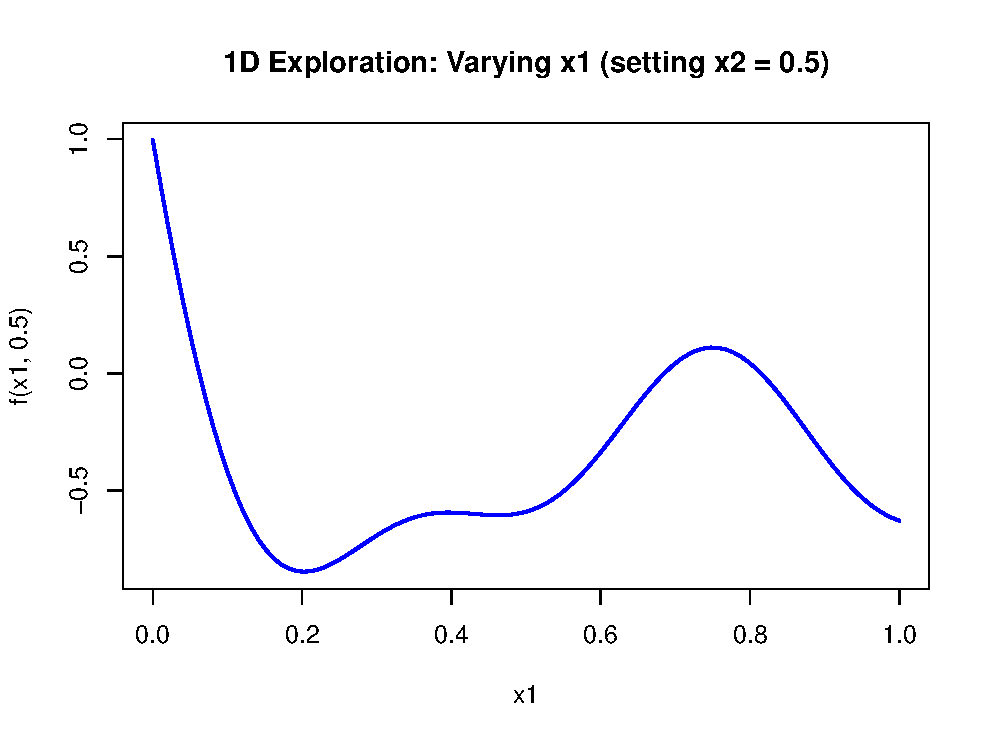
\includegraphics[width=0.45 \textwidth]{1D Exploration.pdf}
    \caption{1D Exploration of the Rescaled Branin-Hoo Function}
    \label{fig:1D Exploration}
\end{figure}

\noindent At $x_1 \approx 0.7$, there is a peak, corresponding to the proximity to one of the minima at $x_1 \approx 0.698$, but since $x_2 = 0.5$ and not $0.818$, it is not at the exact global minimum. This plot can also be used to check how well the emulator matches the actual function in 1D. The following exploration stage involved looking at the function's 2D contour plot:

\begin{figure}[H]
    \centering
    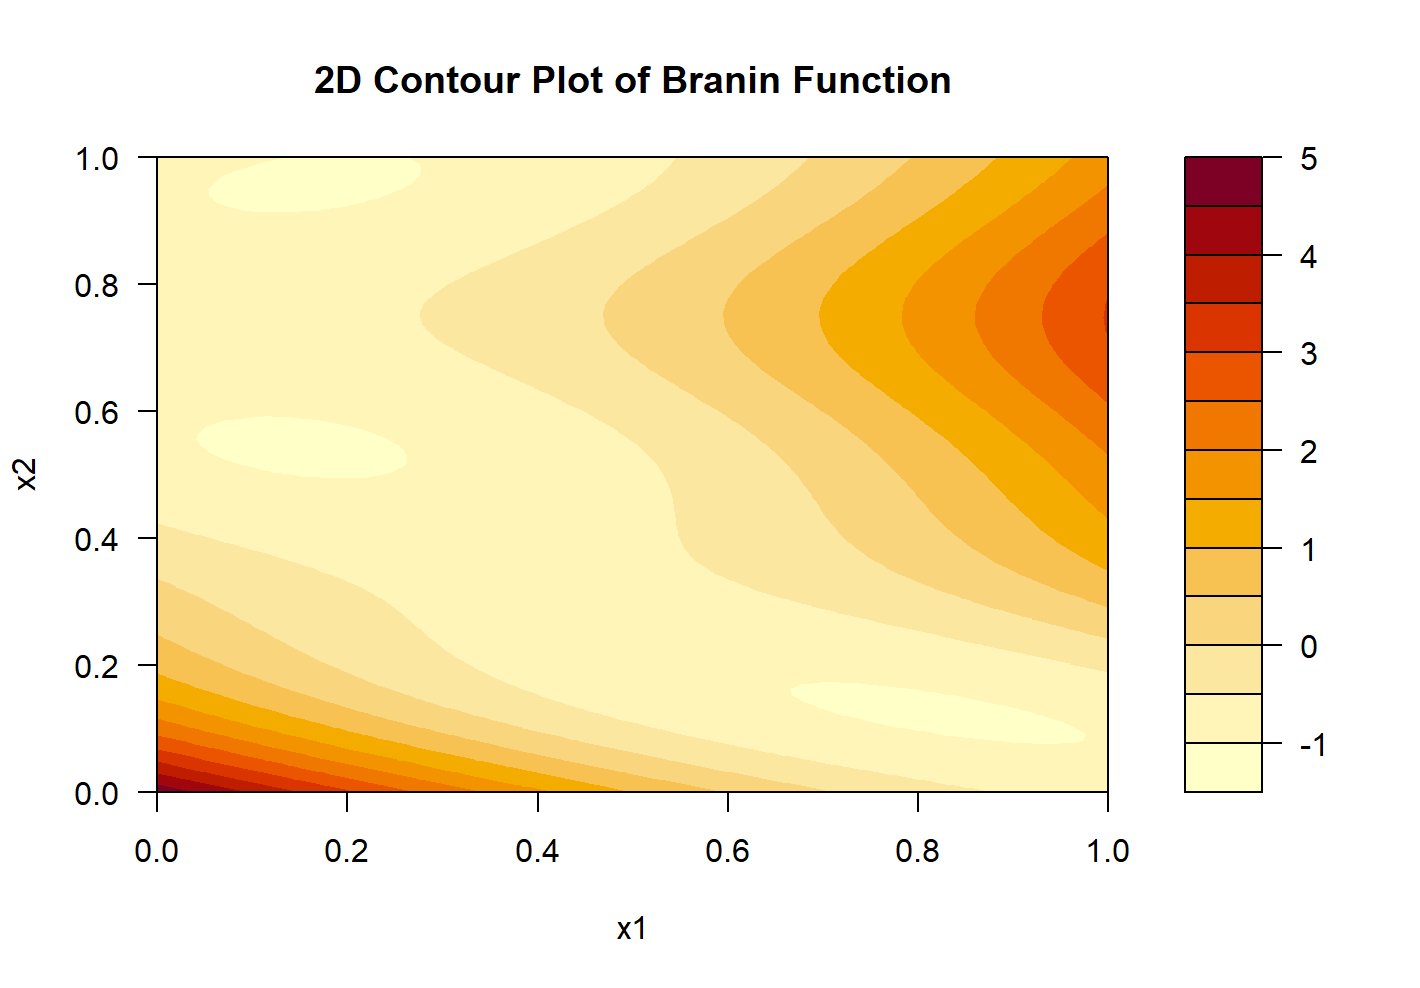
\includegraphics[width=0.55\textwidth]{2D Contour Plot.png}
    \caption{2D Contour Plot}
    \label{fig:2D Contour}
\end{figure}

\noindent The curved contours in \ref{fig:2D Contour} show how both inputs interact, with all 3 of its global minima shown in the light yellow areas. This plot helps because it gives the ``gold standard" of what Bayes Linear Emulation should be aiming for if the true function is available.

\section{Bayes Linear Emulation}

\subsection{Theory}
Before applying Bayes Linear Emulation (BLE), it is important to understand its theory. Given data containing simulator outputs \( D \), from inputs \( x_D = (x_1, x_2, \dots, x_n) \), BLE predicts the output \( f(x) \) at new points \( x_P \) by updating prior expectations and variances through a BL adjustment:

\begin{equation*}
\begin{aligned}
E_D[f(x)] &= E[f(x)] + \text{Cov}[f(x), D] \text{Var}[D]^{-1}(D - E[D]), \hspace{0.25em} \text{and} \\
\text{Var}_D[f(x)] &= \text{Var}[f(x)] - \text{Cov}[f(x), D] \text{Var}[D]^{-1} \text{Cov}[D, f(x)],
\end{aligned}
\end{equation*}


\noindent where $E_D[f(x)]$ and $\text{Var}_D[f(x)]$ are the expectation and variance for $f(x)$,
adjusted by data $D$ and \( \text{Cov}[f(x), D] \) is the covariance between new predictions and true data.\cite{vernon2024} These performances are then evaluated through diagnostics:

\begin{equation*}
    S_D[f(x)] = \frac{E_D[f(x)] - f(x)}{\sqrt{\text{Var}_D[f(x)]}},
\end{equation*}

\noindent or, in other words, \( S_D[f(x)] \) is the emulator's adjusted expectation subtracted from the true function value \( f(x) \), normalised by the emulator's adjusted variance. 

\noindent BLE comes with a few advantages:

\begin{itemize}
    \item Computational Efficiency: They provide predictions of $f(x)$ in the form of the adjusted expectation and variance rapidly.\cite{vernon2024} 
    \item Flexibility: The method accommodates uncertainty, providing useful approximations even with limited simulator runs.\cite{vernon2024}
\end{itemize}

\noindent Ultimately, BLE can be scaled to apply to large datasets where full Bayesian approaches may be less efficient. However, BLE has several limitations that can affect its accuracy and applicability:

\begin{itemize}
    \item Covariance Dependence: Part of the accuracy of a BLE depends on the chosen covariance term. A poor choice results in unreliable predictions.

    \item Non-Gaussian Sensitivity: BLE relies on the Normal distributional assumptions of Gaussian Processes (GPs), which may not hold, hence making these estimates somewhat untrustworthy.\cite{vernon2024}
\end{itemize}

\subsection{Emulation Preparation}
To prepare the function for Emulation, a few normalisation steps were carried out. These scale the input parameters to the $[0,1]$ range, and these become the new emulator inputs. Here is how it is done throughout the code:

\begin{itemize}
    \item The 2D emulator rescales inputs by dividing them by \( \theta \).
    \item The rescaled Branin-Hoo function already assumes inputs \( x_1 \) and \( x_2 \) are in the \([0, 1]\) range due to its normalised form.
    \item The design points generated using \texttt{randomLHS} are already normalised. 
\end{itemize}

\noindent All of these adjustments ensured input data compatibility with emulator training.

\section{1D Emulation}
\ref{fig:1d_emulator} shows the resulting output of the 1D emulator. The emulator predictions (in blue)
closely plot like the Branin-Hoo function. The narrow uncertainty bounds (in red) show the deviation between predicted and actual outputs. These minimal bounds and the emulator output smoothness indicate that the emulator captures the relationship between $x_1$ and $f(x_1, 0.5)$ mostly well. There are 2 noteworthy areas of uncertainty, though, which are the minima at $x_1 \approx 0.2$ and $x_1 \in [0.9,1.0]$, as shown by their wider prediction intervals.

\begin{figure}[H]
    \centering
    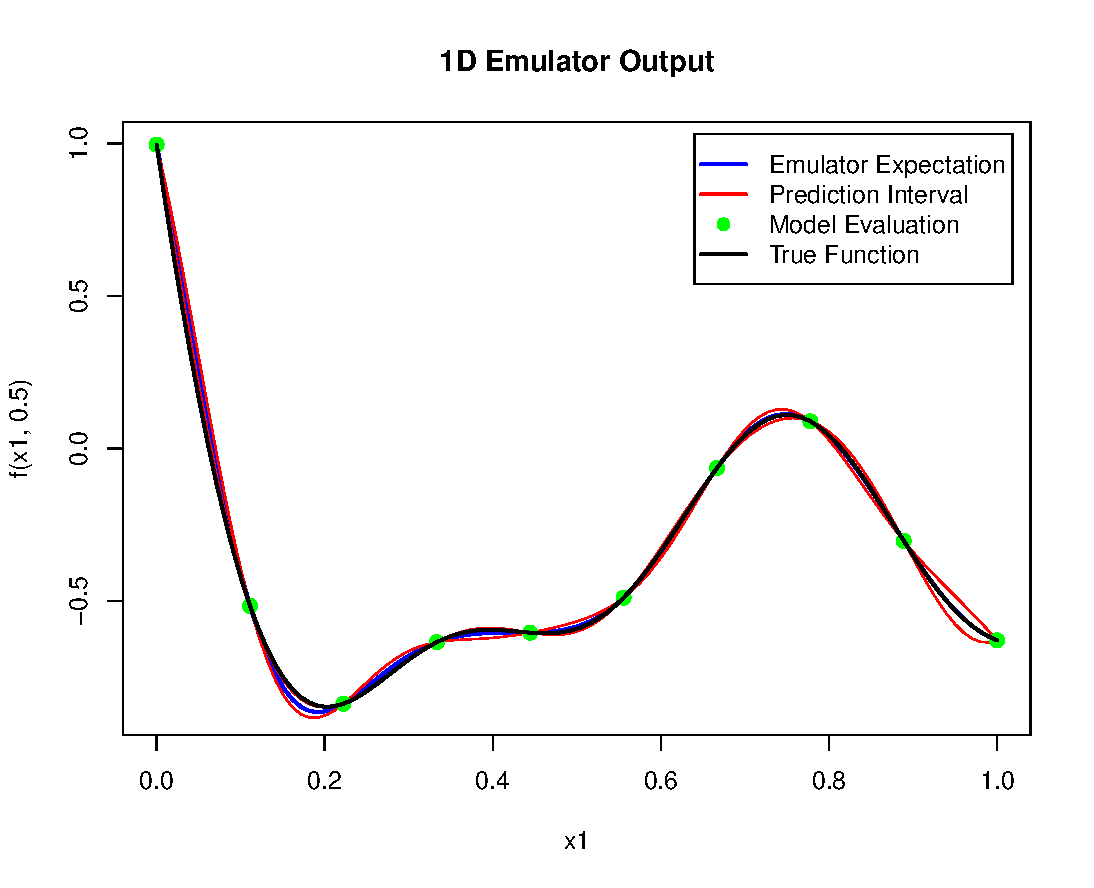
\includegraphics[width=0.6\textwidth]{1D Emulation.pdf}
    \caption{1D Emulator Output showing predictions and uncertainty bounds.}
    \label{fig:1d_emulator}
\end{figure}

\section{2D Emulation}
While 1D Emulation tests emulator performance, it does not consider a function's full complexity, which depends on the interaction between $x_1$ and $x_2$. To address this, 2D Emulation considers both parameters simultaneously, allowing the emulator to model their combined effects.

\subsection{Latin Hypercube Design}
Before delving into 2D Emulation, understanding how it can be applied is essential. This report will apply it through Latin Hypercube Designs (LHDs), and here is how it works:

\noindent For $m$ input dimensions, a LHD for $n$ runs, is formed by:
\begin{enumerate}
    \item Dividing up the range of each input $x_j$ into $n$ equally sized intervals, and then
    
    \item Placing the $n$ runs so that each of the $n$ intervals, for each of the inputs $x_j$, has exactly one run in it.\cite{vernon2024}
    
    \item This is done in turn for each of the $m$ dimensions of the input space, i.e. repeat for $x_j$ with $j = 1, \ldots, m$.\cite{vernon2024}
    
    \item Then either:
    \begin{itemize}
        \item \textbf{Type 1:} add $1/(2n)$ to each $x_j^{(k)}$ entry to recentre intervals' middle points: $\{0, 1/n), [1/n, 2/n), \ldots, [(n-1)/n, 1)\},$
        or
        \item \textbf{Type 2:} add random i.i.d. uniform draws $u_{jk} \sim U[0, 1/n]$ to each entry $x_j^{(k)}$ to randomly sample each point from its chosen $m$ dimensional ``box''.\cite{vernon2024}
    \end{itemize}
\end{enumerate}

\noindent Type 2 is considered beneficial for several reasons; for example, the extra randomness avoids issues due to function periodicity.\cite{vernon2024}

\subsection{Extending to 2D}
Here is the application of 2D Emulation to the Branin-Hoo function:

\begin{figure}[htbp]
    \centering
    % Row 1
    \begin{subfigure}[b]{0.47\textwidth}
        \centering
        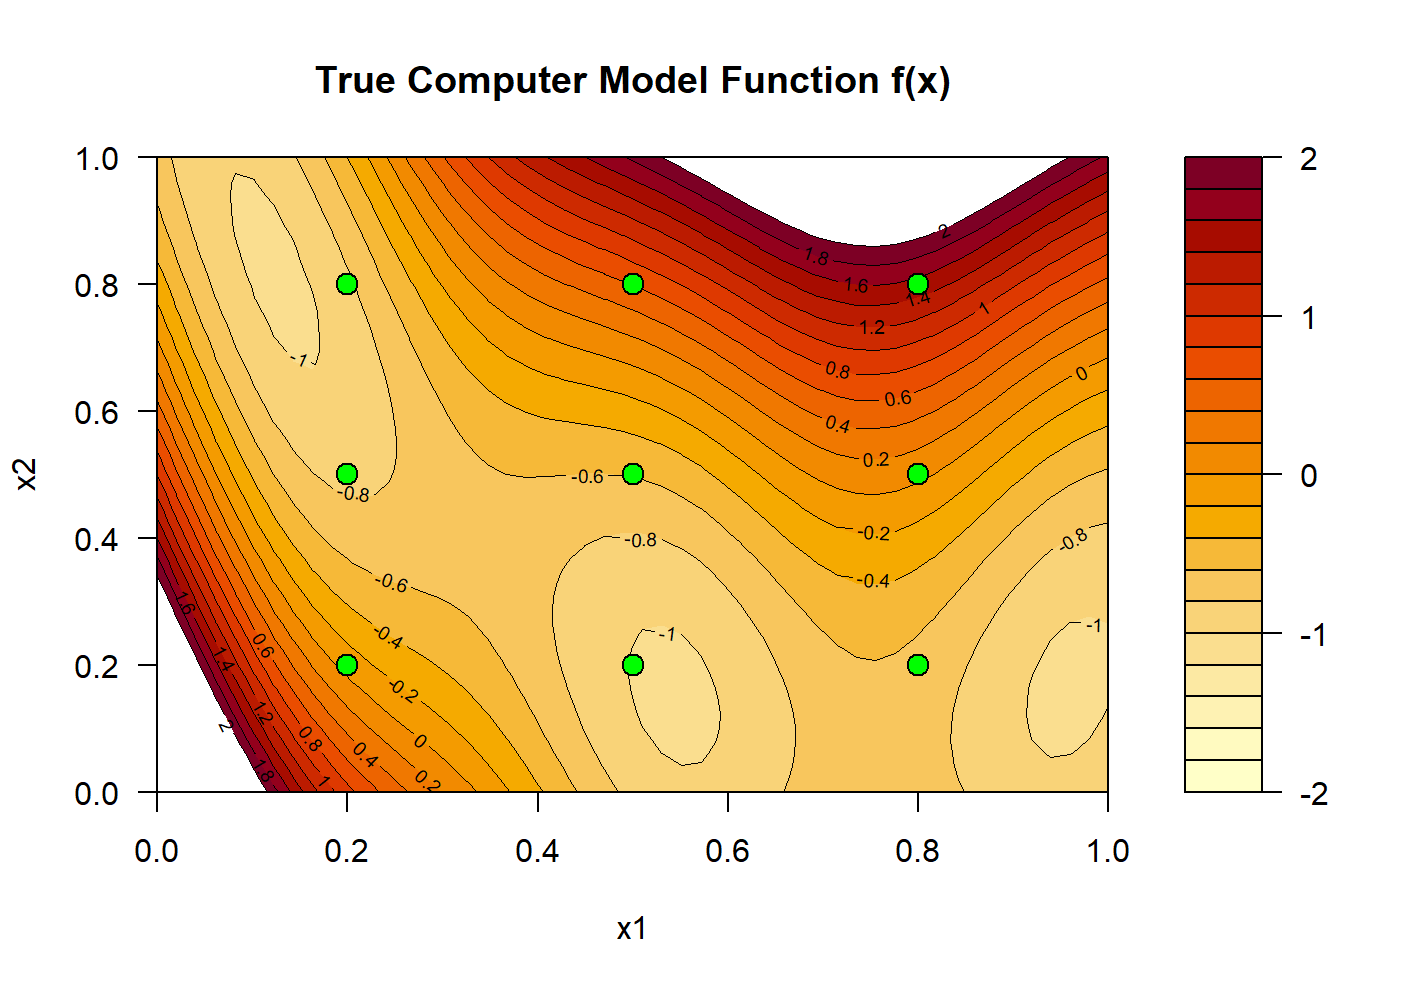
\includegraphics[width=\textwidth]{2D True Model.png}
        \caption{2D True Model}
        \label{fig:true_model}
    \end{subfigure}
    \hfill
    \begin{subfigure}[b]{0.47\textwidth}
        \centering
        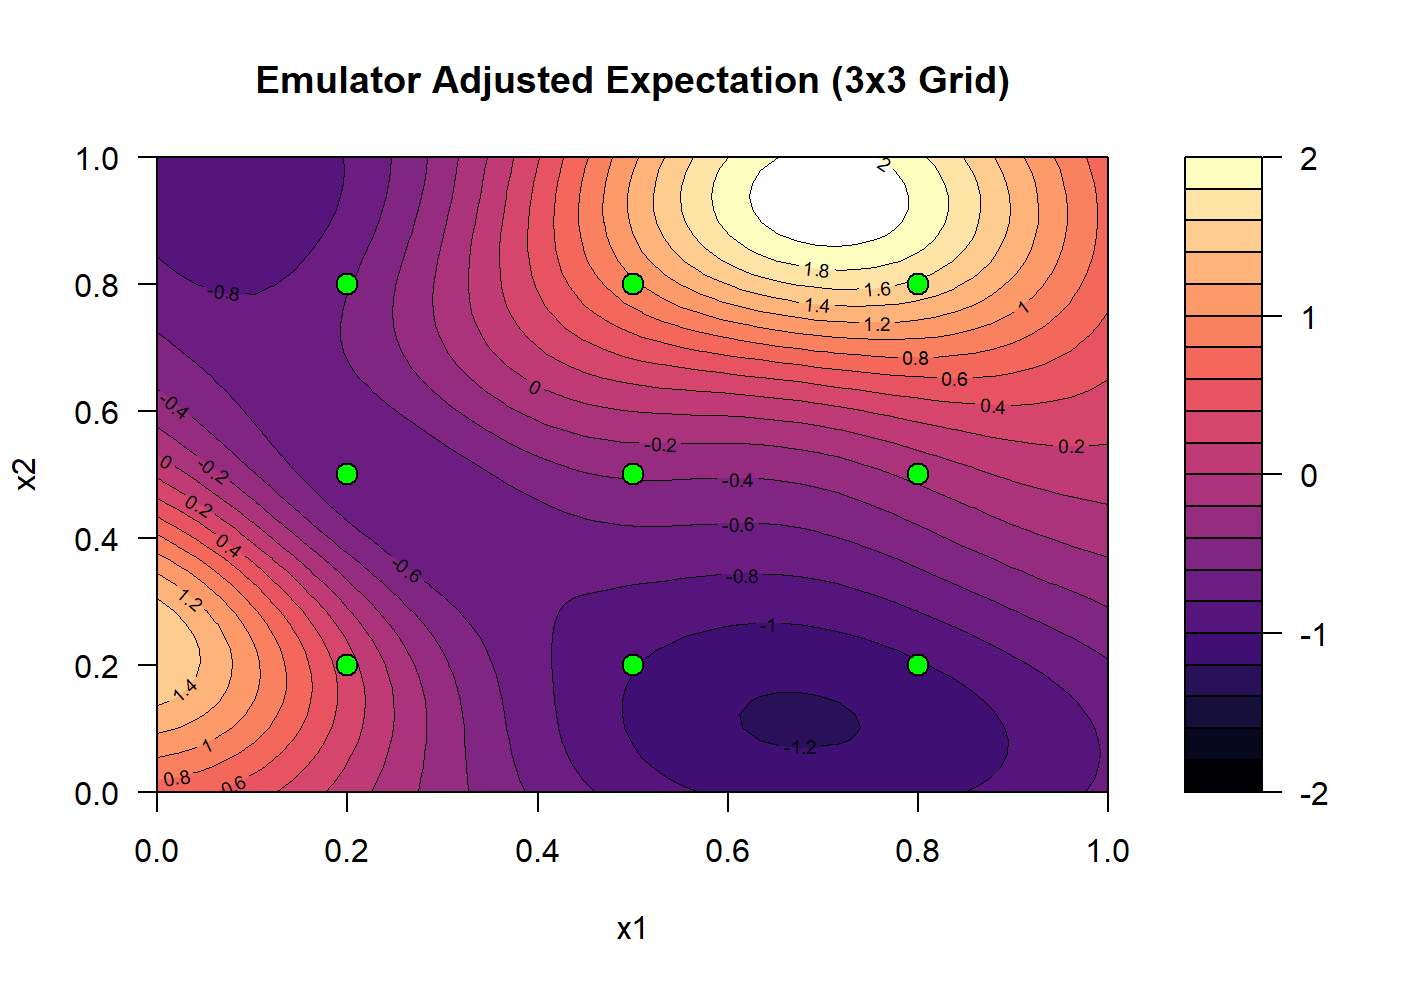
\includegraphics[width=\textwidth]{2D Emulator Expectation.png}
        \caption{2D Emulator Expectation}
        \label{fig:expectation}
    \end{subfigure}

    % Row 2
    \begin{subfigure}[b]{0.47\textwidth}
        \centering
        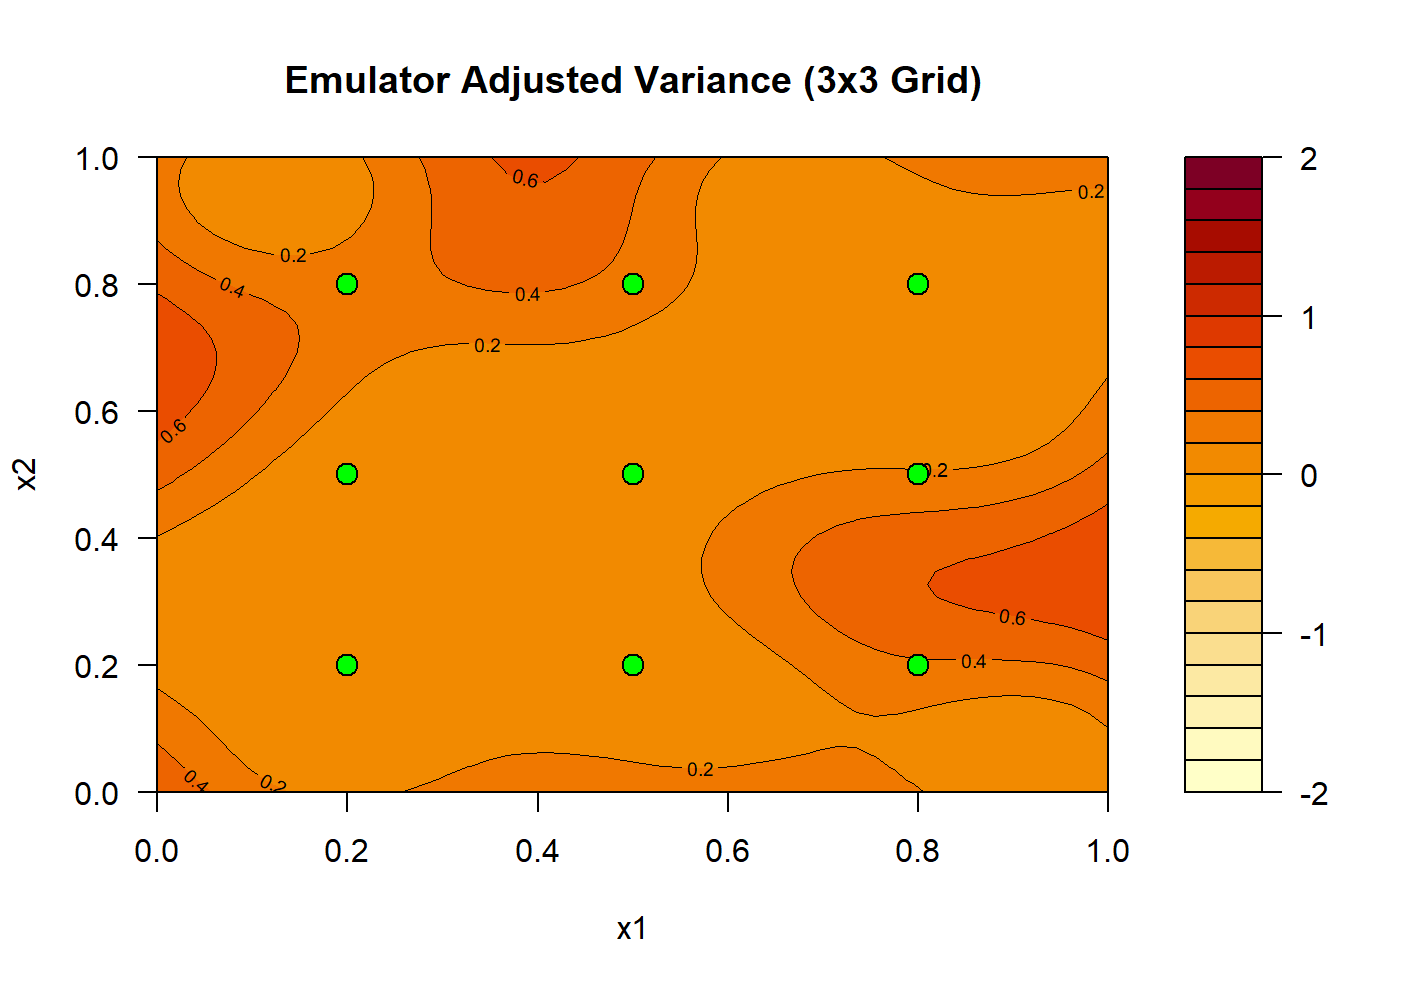
\includegraphics[width=\textwidth]{2D Emulator Variance.png}
        \caption{2D Emulator Variance}
        \label{fig:variance}
    \end{subfigure}
    \hfill
    \begin{subfigure}[b]{0.47\textwidth}
        \centering
        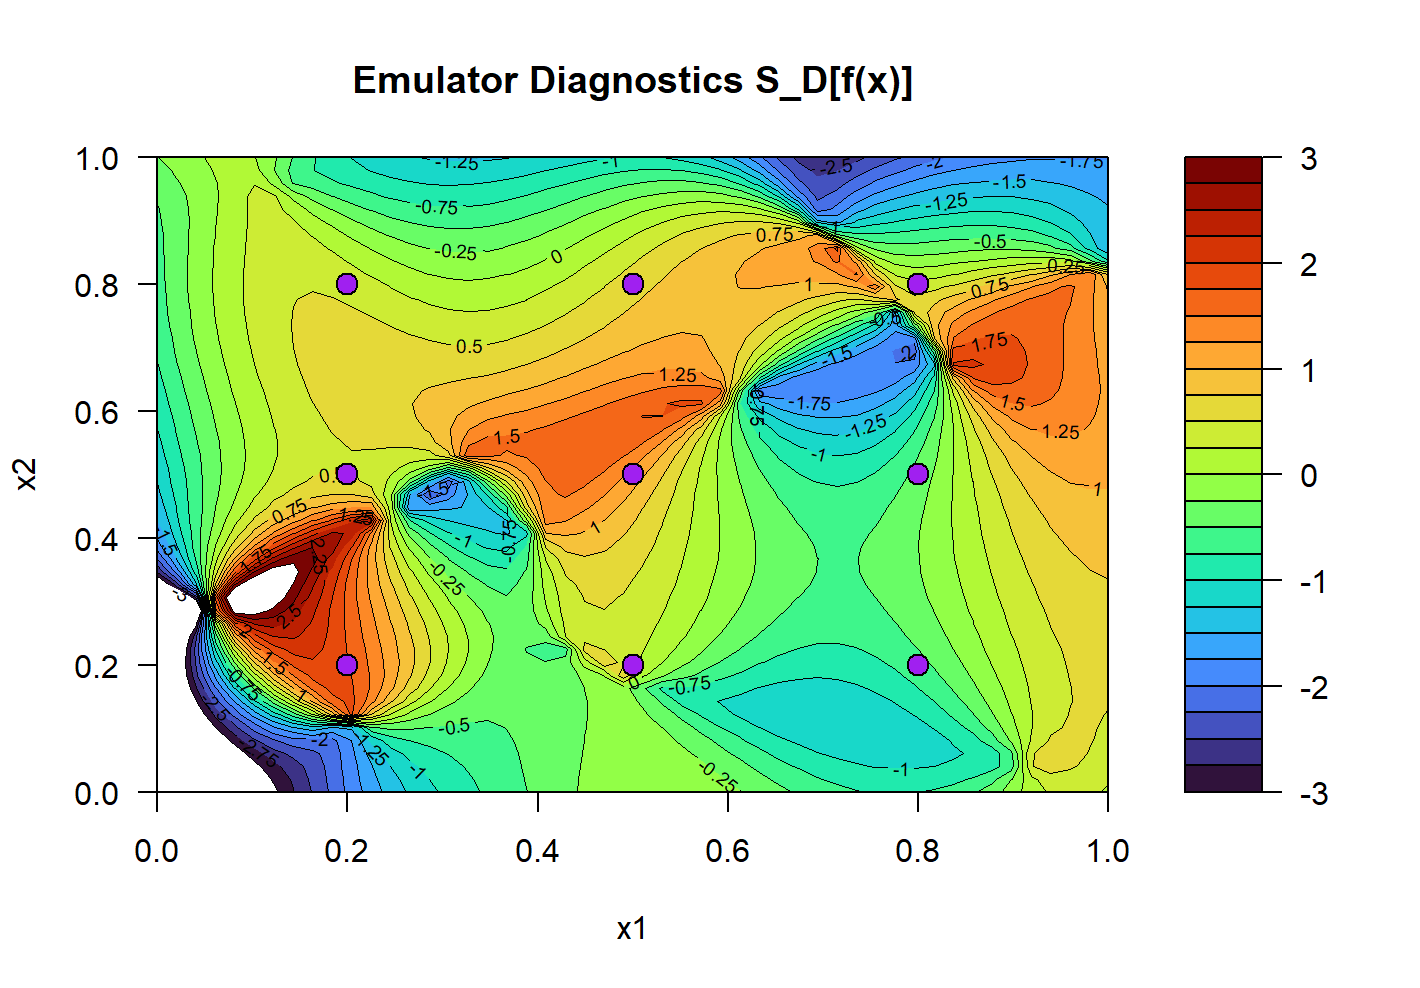
\includegraphics[width=\textwidth]{2D Diagnostics.png}
        \caption{2D Diagnostics}
        \label{fig:diagnostics}
    \end{subfigure}

    \caption{Comparison of 2D Emulator and True Model Outputs}
    \label{fig:comparison}
\end{figure}


\noindent These plots help to assess how well the emulator is performing. The contour lines, in general, represent regions of constant values, with tighter spacing reflecting more rapid value changes. Here are key insights from this set of plots:

\begin{itemize}
    \item The true model, \ref{fig:true_model}, is used to refine BLE by focusing sampling near minima and using fewer points in flatter regions. It is used over \ref{fig:2D Contour} as the emulator only has limited training data, like the true model, avoiding unfair penalisation.
    
    \item \ref{fig:expectation} displays the 2D emulator's expectation. Compared to the true model, the grid points are largely accurate. However, there are some inaccuracies; for example, at $(0.5,0.5)$, its predicted is 0.4 while its actual is 0.6. 

    \item \ref{fig:variance} shows the 2D emulator's variance. The grid points here mainly have low variance, indicating estimate confidence. However, in the top left and bottom right regions, these variances are higher, so sampling should be focused here.

    \item The 2D emulator's diagnostics, see \ref{fig:diagnostics}, identify regions where additional training points may be necessary to refine the emulator's accuracy. The grid points largely display accurate emulator modelling with the only critique being at these points, the emulator is prone to slight overestimation.

\end{itemize}

\noindent Overall, these plots show that the emulator performs well but could benefit from additional training points and further tuning in high-gradient areas, and this is where multi-wave history matching comes in.

\section{Multi-Wave History Matching}

\subsection{History-Matching and Implausibility}
History Matching is an iterative global parameter search method that exploits Emulation to efficiently explore $\mathcal{X}_0$ to find the set of acceptable inputs $\mathcal{X}$.\cite{vernon2024} It compares model outputs with observed data to identify regions in the parameter space that are consistent with historical observations, hence refining model predictions and reducing uncertainty. History matching typically proceeds as follows: First, build an emulator of the model.
Then, calculate implausibility, $I$, across the parameter space, where:

\begin{equation*}
    I^2 (x) = \frac{\left(\text{E}_D[f(x)] - z \right)^2}{\text{Var}_D[f(x)] + \text{Var}[\epsilon] + \text{Var}[e]}. 
\end{equation*}
    
\noindent In this formula, $z$ is the observed emulator value, $\text{Var}[\epsilon]$ is the model discrepancy variance and $\text{Var}[e]$ is the observation error variance.

Next, exclude regions where \( I(\mathbf{x}) > I_{\text{threshold}} \) as they are set as unlikely to produce acceptable matches. This process is repeated iteratively, refining the parameter space in successive waves until only plausible input regions remain.\cite{andrianakis2015bayesian} 

Implausibility is central to history matching. It is a measure that determines whether the input $\mathbf{x}$ is likely to result in an output that will match the observations.\cite{andrianakis2015bayesian}

\subsection{Multi-Wave History Matching and Implausibility Analysis}
Instead of filtering the parameter space once, multi-wave history matching is performed iteratively across multiple waves. Each wave refines the emulator and updates the non-implausible parameter space before proceeding to the next iteration.\cite{salter2016comparison} Early waves may have larger uncertainties, but later waves reduce these uncertainties by focusing emulator training on the non-implausible parameter space.\cite{salter2016comparison} Here were the main results of applying Multi-Wave History Matching onto the rescaled Branin-Hoo Function:

\begin{figure}[H]
    \centering
    % Row 1
    \begin{subfigure}[b]{0.49\textwidth}
        \centering
        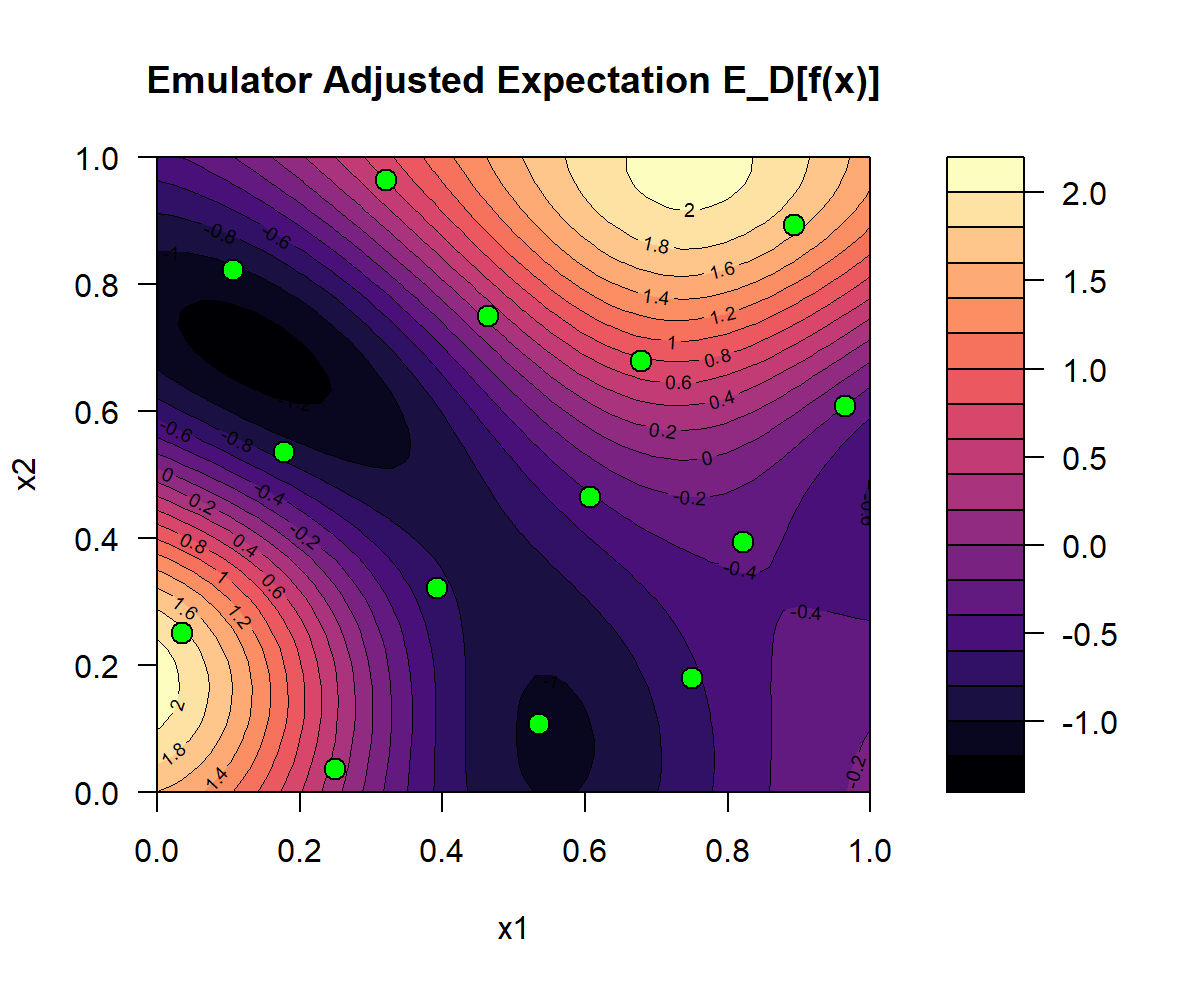
\includegraphics[width=\textwidth]{Wave 1 Emulator Expectation.png}
        \caption{Wave 1 Emulator Expectation}
        \label{fig:Wave 1 Emulator Expectation}
    \end{subfigure}
    \hfill
    \begin{subfigure}[b]{0.49\textwidth}
        \centering
        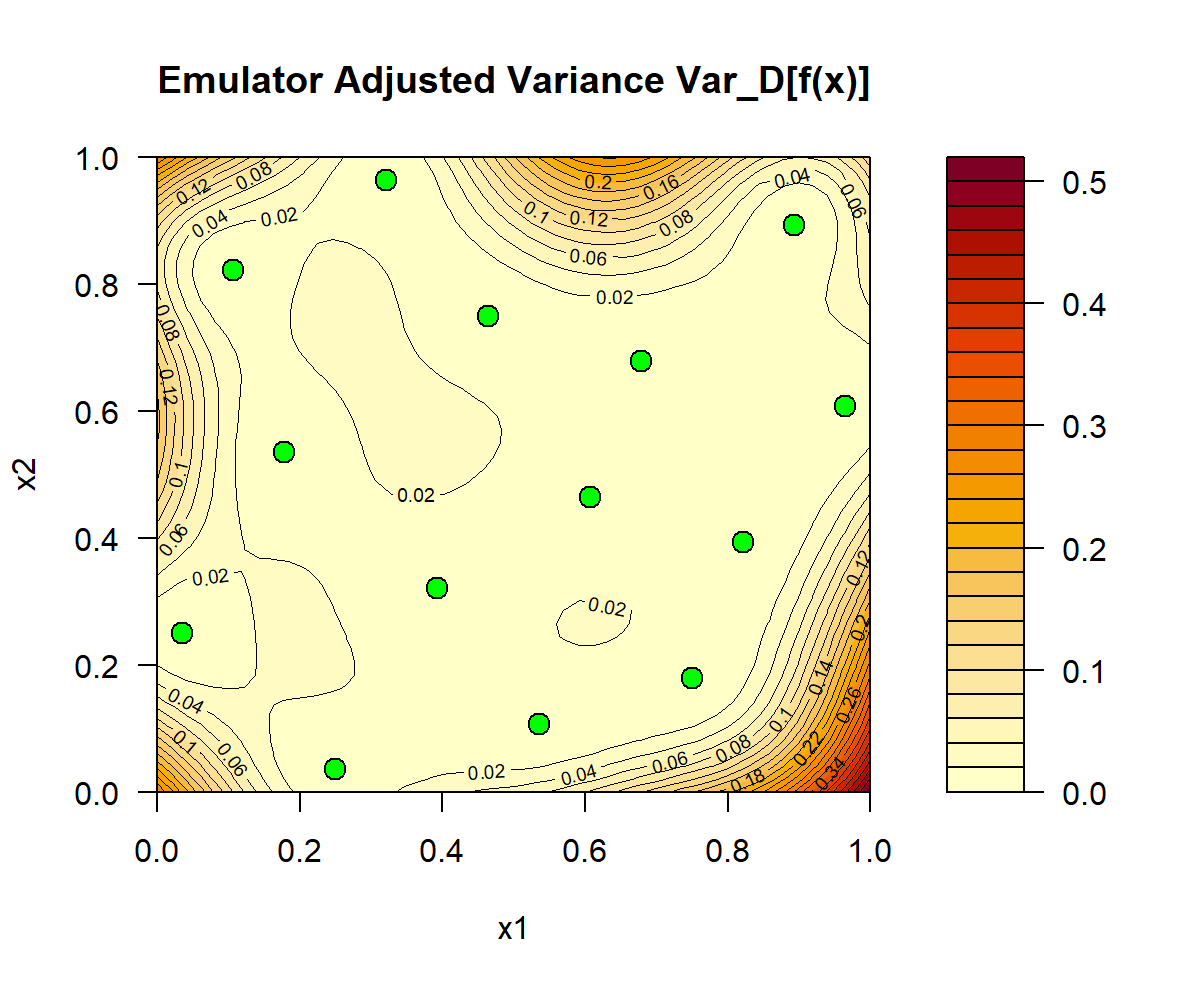
\includegraphics[width=\textwidth]{Wave 1 Emulator Variance.png}
        \caption{Wave 1 Emulator Variance}
        \label{fig:Wave 1 Emulator Variance}
    \end{subfigure}

    % Row 2
    \begin{subfigure}[b]{0.49\textwidth}
        \centering
        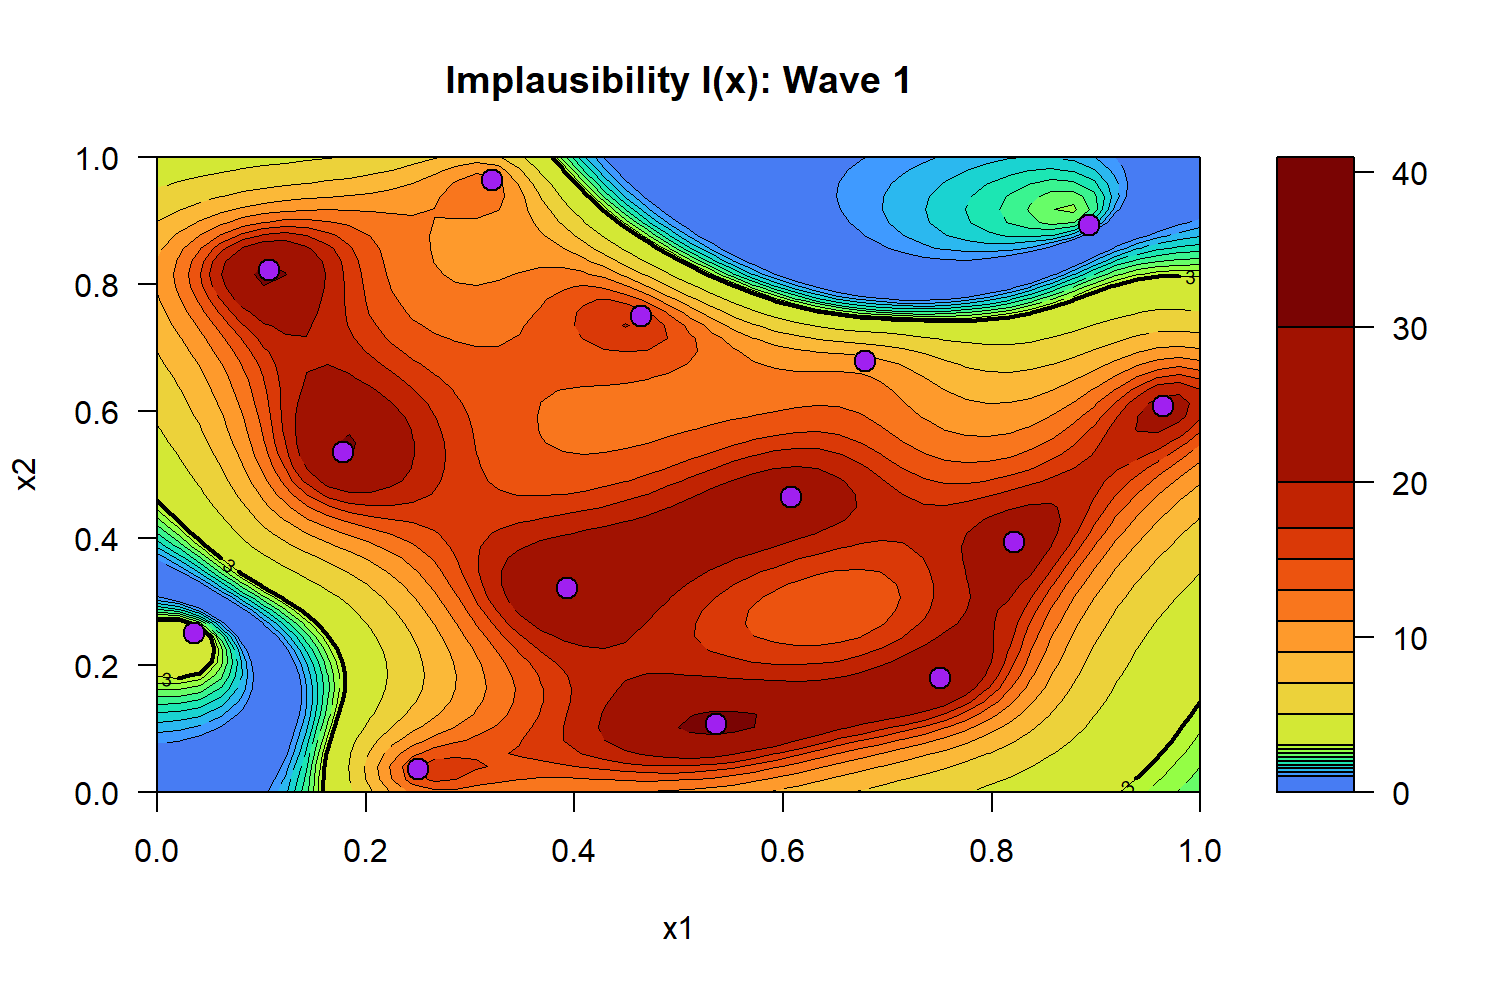
\includegraphics[width=\textwidth]{Wave 1 Implausibility.png}
        \caption{Wave 1 Implausibility}
        \label{fig:Wave 1 Implausibility}
    \end{subfigure}
    \hfill
    \begin{subfigure}[b]{0.49\textwidth}
        \centering
        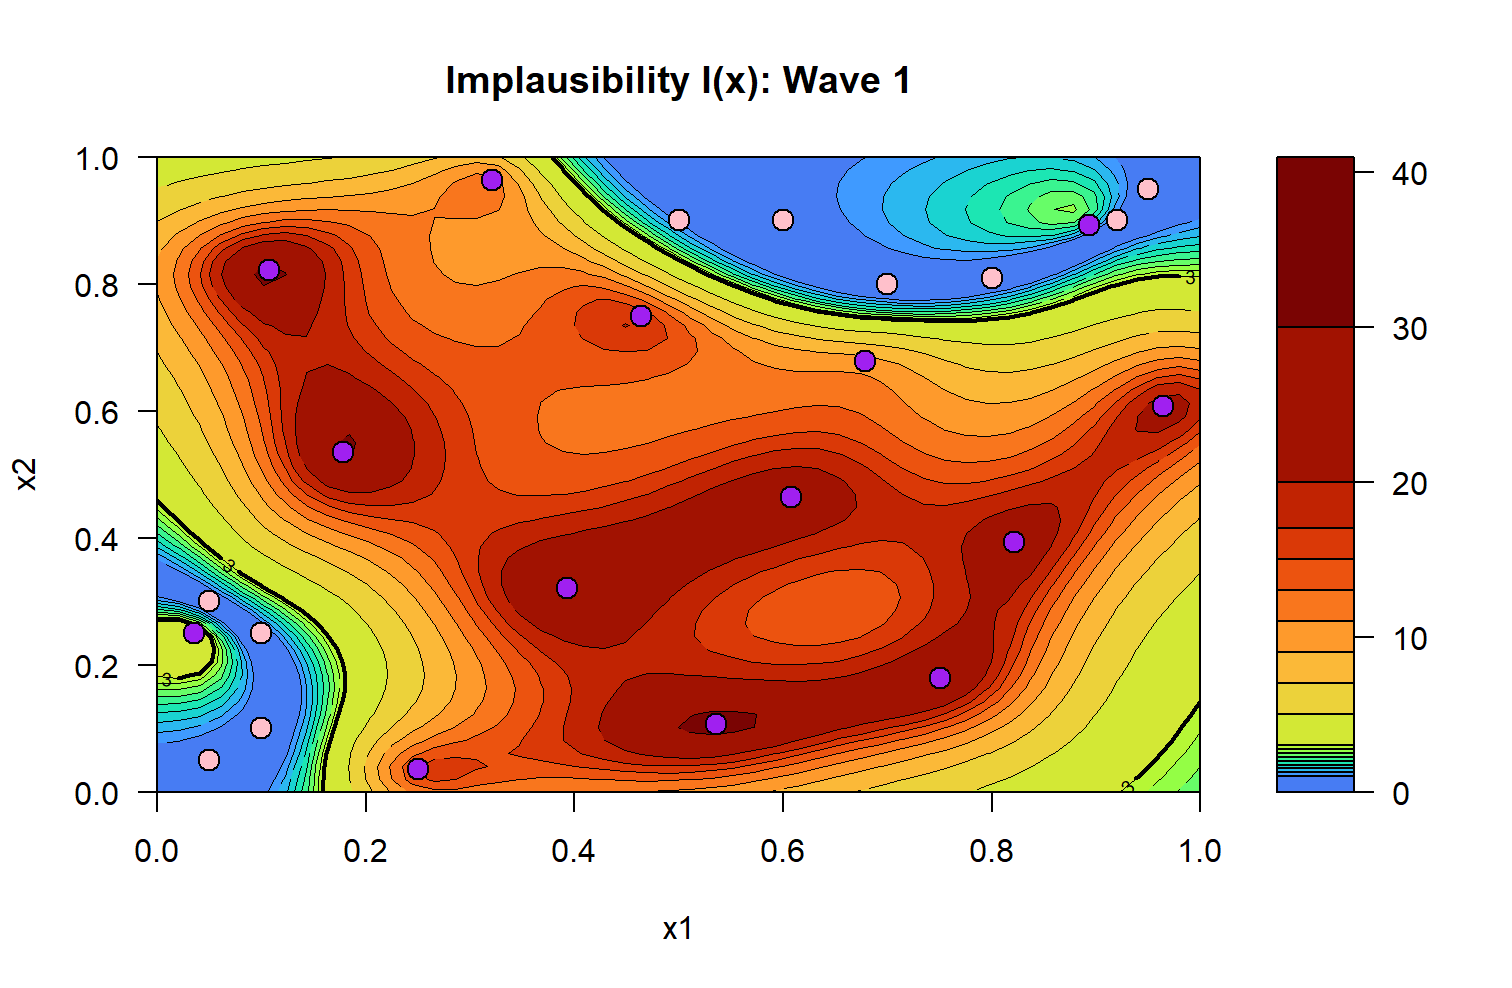
\includegraphics[width=\textwidth]{Current Runs vs. Unevaluated Wave 2 Runs.png}
        \captionsetup{font=footnotesize} 
        \caption{Current Runs vs. Unevaluated Wave 2 Runs}
        \label{fig:Current Runs vs. Unevaluated Wave 2 Runs}
    \end{subfigure}

    \caption{Wave 1 History-Matching}
    \label{fig:Wave 1 History-Matching}
\end{figure}

\begin{itemize}
    \item \ref{fig:Wave 1 Emulator Expectation} shows the emulator’s predicted expectation. There is a minimum starting from $x_2 \in [0.8, 1.0]$ and $x_1 = 0$ and ending at $x_1 \in [0.4, 0.7]$ and $x_2 = 0$, indicating significant variation. Also, the Branin-Hoo function increases towards the top-right, suggesting a gradient.
    \item \ref{fig:Wave 1 Emulator Variance} shows the emulator's uncertainty, representing confidence in predictions. Variance is low across most regions, indicating confidence in the emulator's predictions. Also, uncertainty is higher near the edges where no training points exist.
    \item \ref{fig:Wave 1 Implausibility} shows the emulator's implausibility, assessing emulator model fit. There are 2 clear areas of low implausibility, which the next wave will look at by taking design points in these regions.
    \item \ref{fig:Current Runs vs. Unevaluated Wave 2 Runs} shows the locations of the first-wave runs (purple) and the 10 new second-wave candidate points (pink). The Wave 2 runs are mainly in low implausibility regions to help the emulator refine the model.
\end{itemize}

\begin{figure}[H]
    \centering
    \begin{subfigure}{0.49\textwidth}
        \centering
        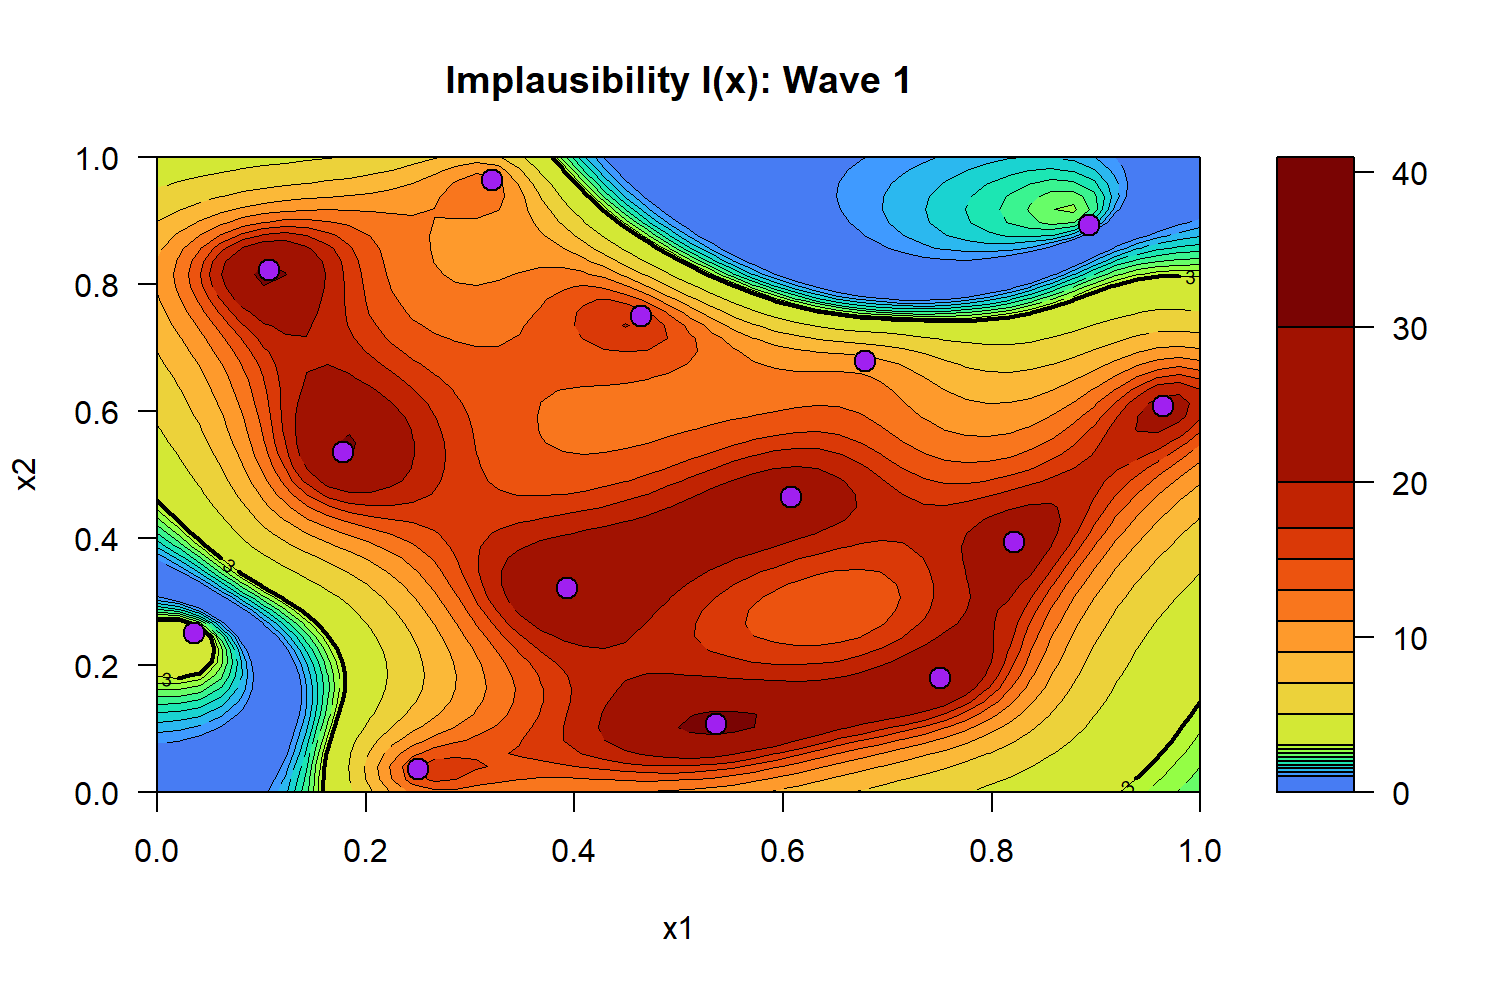
\includegraphics[width=\linewidth]{Wave 1 Implausibility.png}
        \caption{Wave 1 Implausibility}
        \label{fig:wave1}
    \end{subfigure}
    \hfill
    \begin{subfigure}{0.49\textwidth}
        \centering
        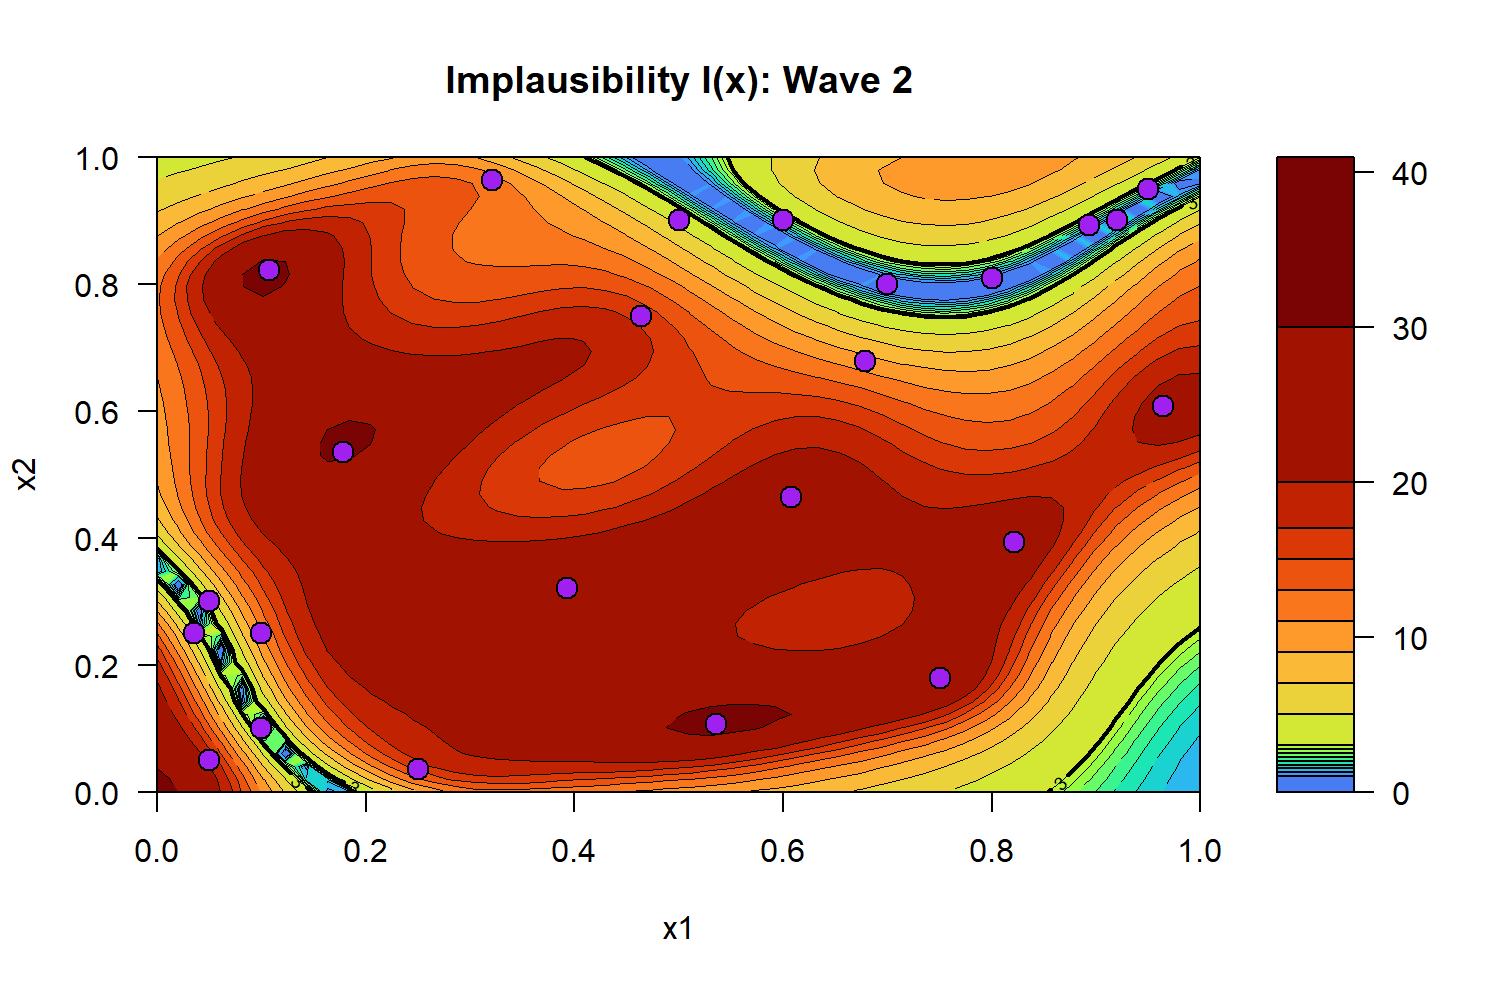
\includegraphics[width=\linewidth]{Wave 2 Implausibility.png}
        \caption{Wave 2 Implausibility}
        \label{fig:wave2}
    \end{subfigure}
    
    \begin{subfigure}{0.6\textwidth}
        \centering
        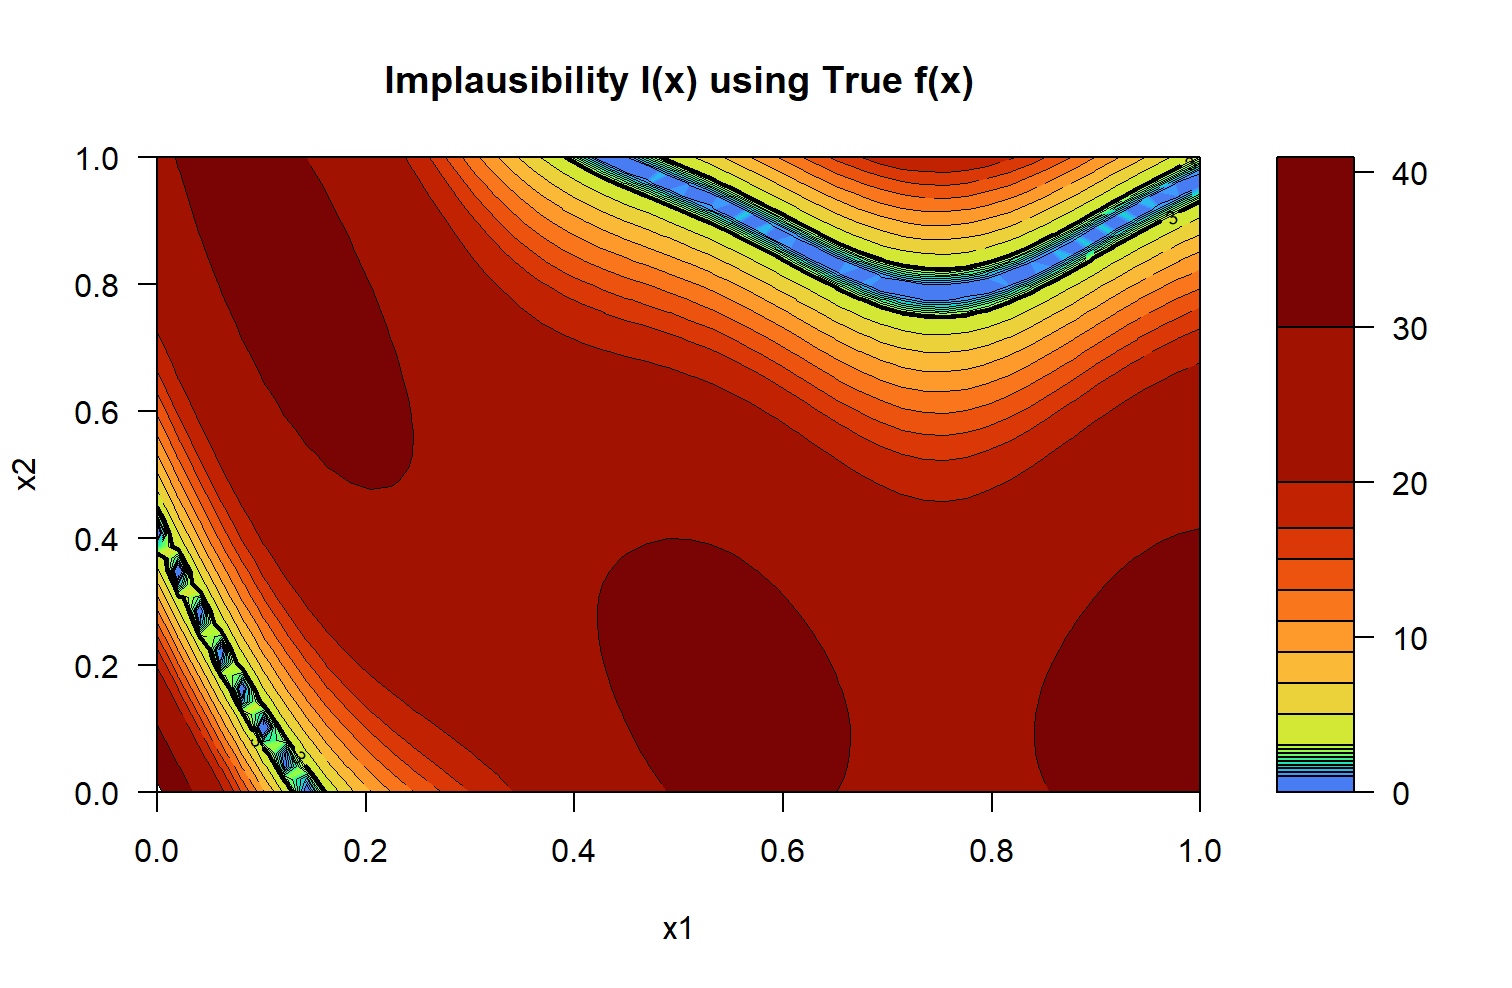
\includegraphics[width=\linewidth]{Wave Implausibility I(x) using True f(x).png}
        \caption{Implausibility I(x) using True $f(x)$}
        \label{fig:true_implausibility}
    \end{subfigure}
    
    \caption{Comparison of implausibility across Wave 1, Wave 2, and the true function.}
    \label{fig:implausibility_comparison}
\end{figure}

\begin{itemize}
    \item \ref{fig:wave1} is the implausibility after the initial grid points were applied. \ref{fig:wave1} is repeated for direct comparison with \ref{fig:wave2}, which is the implausibility after more grid points are added.
    \item The grid points have been added in key areas of high previous uncertainty along the upper-right and lower-left regions, matching where the true function had low implausibility values.
    \item These plots show how implausibility adjusts as the model explores the parameter space more and more. As shown by the blue region's precision in \ref{fig:wave2}.
    \item There are still some issues, however, as there is a blue region on the bottom right of \ref{fig:wave2}, and this should not be the case. However, this can be fixed with more grid points taken there.
\end{itemize}

\noindent Ultimately, taking more samples in low implausible regions has refined the emulator, leading to better alignment with the true function's implausibility, \ref{fig:true_implausibility}.


\chapter{Conclusion \& Further Research}

\section{Conclusion}
The results presented in Figures \ref{fig:1d_emulator} to \ref{fig:implausibility_comparison} showcase the progression of Emulation from the simple 1D case to multi-wave history matching. The emulator's performance improves with each wave. The implausibility map highlights areas where emulator predictions may require improvements. By iteratively refining the parameter space, the emulator achieved tighter uncertainty bounds and improved observational data alignment on further waves.

By applying simple BLEs for single and multiple inputs, the project highlighted BLE's efficiency in approximating complex functions with limited computational resources. The emulator's performance was visualised through various plots, illustrating the expectation and variance of the emulated functions across the input space. LHD ensured adequate exploration of the parameter space, while the iterative history-matching process allowed for emulator refinement by excluding implausible regions. The results emphasise how Emulation can significantly improve computational models by providing insight into the variability and uncertainty of model outputs. Through multi-wave history matching, the emulator successfully adapted to new data points, improving its accuracy and narrowing down the plausible parameter space.

\section{Further Research}
Although this project covered BL Emulators in depth, there are several avenues for further research. While BLE is more computationally efficient, Gaussian Process Emulation (GPE) provides a full probabilistic specification across functions, meaning the posterior remains a full Gaussian Process. \cite{vernon2024} Future research could involve applying GPE using packages such as \texttt{DiceKriging}. Comparing BLE and GPE provides insights into how the posterior distribution influences model predictions. 
 Future work could also involve applying the developed emulator to real-world cases, such as in climate modelling.

% Change bibliography numbering format
\makeatletter
\renewcommand\@biblabel[1]{#1.} % Change numbering style to 1.
\makeatother
\bibliographystyle{unsrt}
\bibliography{references}

\end{document}

\end{document}
